% TODO:
%
% * update the RV numbers
% * redo the RV fit with the latest CKS points
% * email to JNW
% * email to full collaborator list
% * add any missing CPS coauthors
% * check if it was really only 5 CPS points in knutson's paper
%
%%%%%%%%%%%%%%%%%%%%%%%%%%%%%%%%%%%%%%%%%%%%%%%%%%%%%%%%%%%%%%%%%%%%%%%%%%%%%%%

\documentclass[RNAAS]{aastex62}
\usepackage{amsmath,amstext,amssymb}
\usepackage[T1]{fontenc}
\usepackage{apjfonts}
\usepackage[figure,figure*]{hypcap}
\usepackage{graphics,graphicx}
\usepackage{hyperref}

\begin{document}

\title{WASP-4 is accelerating towards the Earth}

\correspondingauthor{L. G. Bouma}
\email{luke@astro.princeton.edu}

\author[0000-0002-0514-5538]{L. G. Bouma}
\affiliation{ Department of Astrophysical Sciences, Princeton
University, 4 Ivy Lane, Princeton, NJ 08540, USA}
%
\author[0000-0002-4265-047X]{J. N. Winn}
\affiliation{ Department of Astrophysical Sciences, Princeton
University, 4 Ivy Lane, Princeton, NJ 08540, USA}
%
\author[0000-0001-8638-0320]{A. W. Howard}
\affiliation{Cahill Center for Astrophysics, California Institute of
Technology, Pasadena, CA 91125, USA}
%
\author{H. Knutson}
\affiliation{Division of Geological and Planetary Sciences, California
Institute of Technology, Pasadena, CA 91125, USA}
%
\author[0000-0002-0531-1073]{H. Isaacson}
\affiliation{Astronomy Department, University of California, Berkeley,
CA 94720, USA}
%

%% Note that RNAAS manuscripts DO NOT have abstracts.
%% See the online documentation for the full list of available subject
%% keywords and the rules for their use.
\keywords{Exoplanet tides (497), Exoplanet dynamics (490), Radial velocity 
(1332), Transit timing variation method (1710)}

%% Start the main body of the article. If no sections in the 
%% research note leave the \section call blank to make the title.

\section{}
%%%%%%%%%%%%%%%%%%%%%%%%%%%%%%%%%%%%%%%%%%%%%%%%%%%%%%%%%%%%%%%%%%%%%%%%%%%%%%%

In recent work we showed that the TESS spacecraft observed the hot
Jupiter WASP-4b transit $\approx 82$ seconds earlier than expected,
under the assumption of a constant orbital period
\citep{bouma_wasp-4b_2019}.  This result was based on transit
times\footnote{ Our timing analysis included data from peer-reviewed
literature for which the times were measured from a single transit,
and for which the midpoint was allowed to be a free parameter. We also
required that the time system be clearly documented. In other words,
we needed to know
whether any heliocentric/barycentric corrections had been performed,
and whether the absolute time system was UTC or TDB.} acquired since
2007 (CITE ALL).  We pointed out that the transit times were best fit
by a timing model with a constant period derivative, and reported a
best-fit decay rate of $\dot{P} = -12.6 \pm 1.2\,{\rm ms\ per\ year}$.
Our interpretation was that the apparent period change could be caused
by any of three scenarios: a decaying orbit, a precessing orbit, and
an orbit being gravitationally perturbed by an outer companion.

Thereafter, \citet{southworth_transit_2019} reported 22 new transit
times for the system, and also found that the entire series of transit
times was consistent with a quadratic ephemeris.  Their interpretation
of the timing variations did not differ in any major respects from our
own, though with their additional data a lower best-fit decay rate was
reported ($\dot{P} = -XX.X \pm X.X\,{\rm ms\ per\ year}$).

A separate study by \citet{baluev_homogeneously_2019} also reported
new light curves. \citeauthor{baluev_homogeneously_2019} analyzed
their newly obtained light curves, along with archival light curves
that were omitted from our analysis due to systematic uncertainties in
the absolute time system.  \citeauthor{baluev_homogeneously_2019}
found that when they used all the available TTV data, the need for a
quadratic ephemeris was present ``at the high $\sim 5-7$ sigma
level''.  However, they pointed out that if they used lower-precision
subsets of the available timing data, the necessity for the quadratic
term decreased.  \citeauthor{baluev_homogeneously_2019} also pointed
out that the precise transit times reported by
\citet{huitson_gemini_2017} were quite important in the time-series.
Overall, \citeauthor{baluev_homogeneously_2019} were not convinced.

We, too, wanted to confirm and understand the timing variation.  One
line of follow-up we mentioned was the need for additional radial
velocity observations.  We acquired them this past season with Keck
HIRES.
After fitting out the hot Jupiter, the residuals now show a strong
linear trend  (Figure~\ref{fig:rv_o_minus_c}).
Specifically, the best-fit radial velocity derivative, $\dot{v}_{\rm
r}$, is
\begin{equation}
  \dot{v}_{\rm r} = - X.XX \pm Y.YY\,{\rm m\,s^{-1}\,day^{-1}}.
\end{equation}
This acceleration towards our line of sight is XXX times faster than 
reported from the 5 points available during the Friends of Hot
Jupiters project \citep{knutson_friends_2014}.
%FoHJ: gammadot = -0.0099^{+0.0052}_{-0.0054}
The updated radial velocity values are available in the
data-behind-the-figure online version of this {\it Note}.

Under the assumption of constant acceleration, $\dot{P} = \dot{v}_{\rm
r} P / c$, so the implied period decrease that should be seen in
transits is $\approx$X.X milliseconds per year.
All the available TTV data show a period decrease of $\approx
8-12\,{\rm ms\ per\ year}$
\citep{bouma_wasp-4b_2019,southworth_transit_2019,baluev_homogeneously_2019}.

It seems quite likely that the line of sight acceleration is to blame
for the apparent decrease of WASP-4b's orbital period.  While further
radial velocity observations of the system should help clarify the
mass and semi-major axis of the companion, it seems unlikely that
further transit observations will yield near-term constraints on
orbital decay.


%%%%%%%%%%%%%%%%%%%%%%%%%%%%%%%%%%%%%%%%%%%%%%%%%%%%%%%%%%%%%%%%%%%%%%%%%%%%%%%
% RNAAS: you get one figure.

\begin{figure}
    \begin{center}
		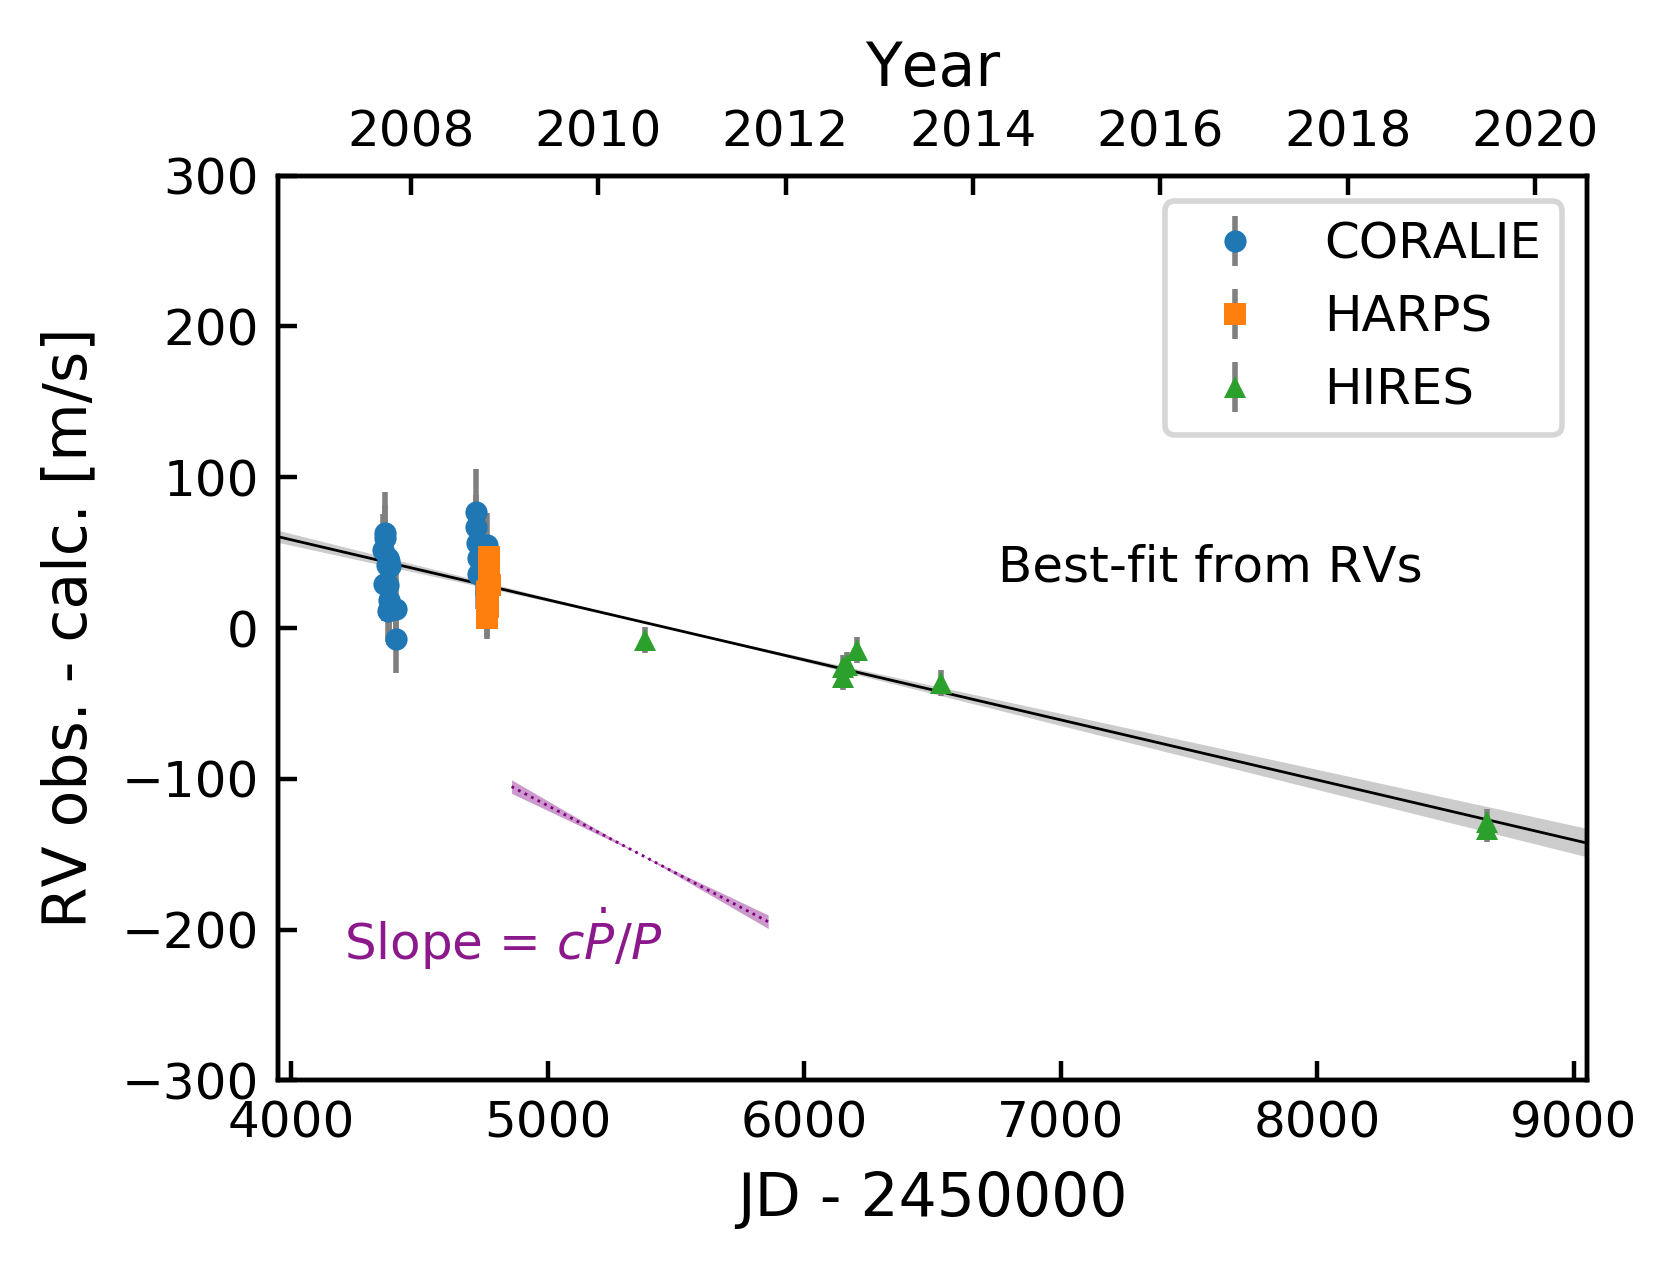
\includegraphics{20190716_rv_fit.png}
    \end{center}
    \vspace{-0.8cm}
    \caption{
      {\bf Radial velocity observations of WASP-4.}
      The orbit of WASP-4b has been subtracted.
      %FIXME: finish writing.
       \label{fig:rv_o_minus_c}
    }
\end{figure}

%%%%%%%%%%%%%%%%%%%%%%%%%%%%%%%%%%%%%%%%%%%%%%%%%%%%%%%%%%%%%%%%%%%%%%%%%%%%%%%

\acknowledgements

%
This paper includes data collected by the TESS mission, which are
publicly available from the Mikulski Archive for Space Telescopes
(MAST).
%
Funding for the TESS mission is provided by NASA's Science Mission
directorate.
%
This research has made use of the NASA Exoplanet Archive, which is
operated by the California Institute of Technology, under contract
with the National Aeronautics and Space Administration under the
Exoplanet Exploration Program.
%
This work made use of NASA's Astrophysics Data System Bibliographic
Services.
%
This research has made use of the VizieR catalogue access tool, CDS,
Strasbourg, France. The original description of the VizieR service was
published in A\&AS 143, 23.
%
This work has made use of data from the European Space Agency (ESA)
mission {\it Gaia} (\url{https://www.cosmos.esa.int/gaia}), processed
by the {\it Gaia} Data Processing and Analysis Consortium (DPAC,
\url{https://www.cosmos.esa.int/web/gaia/dpac/consortium}). Funding
for the DPAC has been provided by national institutions, in particular
the institutions participating in the {\it Gaia} Multilateral
Agreement.
%
\newline
%
\software{
  \texttt{radvel} \citep{fulton_radvel_2018},
}

\bibliographystyle{yahapj}                            
\bibliography{bibliography} 

\end{document}
